\documentclass{standalone}
\usepackage{tikz}
\usepackage{ctex,siunitx}
\usepackage{tkz-euclide}
\usepackage{amsmath}
\usetikzlibrary{patterns, calc}
\usetikzlibrary {decorations.pathmorphing, decorations.pathreplacing, decorations.shapes,}
\begin{document}
\small
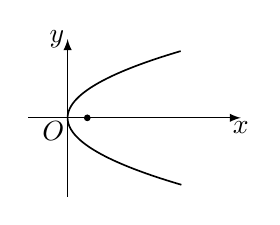
\begin{tikzpicture}[>=latex,scale=1.0,inner sep=1pt]
  \draw[thin,->](-0.5,0)--(2.2,0)node[below]{$x$};
  \draw[thin,->](0,-1)--(0,1)node[left]{$y$};
  \tkzDefPoints{0/0/O,0.25/0/F}
  \draw[semithick,domain=-0.85:0.85,samples=200] plot ({2*\x*\x},{\x});
  \tkzDrawPoints[fill=black](F)
  \tkzLabelPoints[below left](O)
\end{tikzpicture}
\end{document}